\subsection[Il ruolo della Loss nell'addestramento]{Il ruolo della Loss nell'addestramento}


\begin{frame}

	\frametitle{La minimizzazione empirica del rischio}

	\begin{block}{}
		Addestrare un modello significa semplicemente far imparare (determinare) dei buoni valori per tutti i pesi e il bias da esempi etichettati.\\
		\vspace{3mm}
		Nell'apprendimento supervisionato si costruisce un modello esaminando molti esempi e tentando di trovare un modello che riduca al minimo la \textbf{loss}; questo processo è chiamato \textbf{minimizzazione empirica del rischio}.\\
		\vspace{3mm}
		La \textbf{loss} è la penalità per una previsione sbagliata. In altre parole, la \textbf{loss} è un numero che indica la cattiva previsione del modello su un singolo esempio.\\
		\vspace{3mm}
		Se la previsione del modello è perfetta, la \textbf{loss} è zero; in caso contrario, la \textbf{loss} è maggiore di 0. L'obiettivo dell'addestramento di un modello è trovare un insieme di pesi e bias che abbiano una \textbf{loss bassa}, in media, in tutti gli esempi.
	\end{block}

\end{frame}


\begin{frame}

	\frametitle{Un esempio}

	%\begin{block}{}
		Ad esempio, la figura mostra:
		\begin{itemize}
			\item un modello con loss alta a sinistra
			\item un modello con loss bassa a destra
		\end{itemize}

		Nella figura:
		\begin{itemize}
			\item Le frecce rappresentano la loss
			\item Le linee blu rappresentano le previsioni
		\end{itemize}

		\begin{figure}[!htbp]
			\centering
			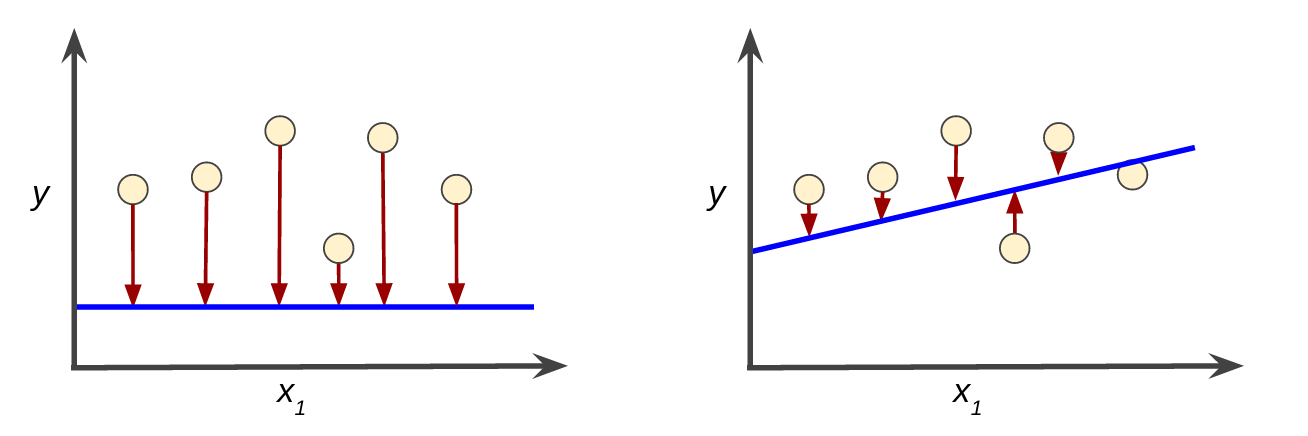
\includegraphics[width=12cm]{images/supervised/training_loss_role/LossSideBySide.png}
			%\caption{Stripe Radar for Fraud Detection}
		\end{figure}

	%\end{block}

\end{frame}


\begin{frame}

	\frametitle{Un esempio: osservazioni}

	%\begin{block}{Osservazioni}
		\begin{itemize}
			\item si può osservare che le frecce nel grafico a sinistra sono molto più lunghe delle loro controparti nel grafico a destra
			\item chiaramente, la retta del grafico di destra è un modello predittivo molto migliore rispetto alla retta del grafico di sinistra
			\item ci si potrebbe chiedere se è possibile creare una funzione matematica, una funzione di \textbf{loss}, che aggreghi le perdite individuali in modo sensato
		\end{itemize}

		\begin{figure}[!htbp]
			\centering
			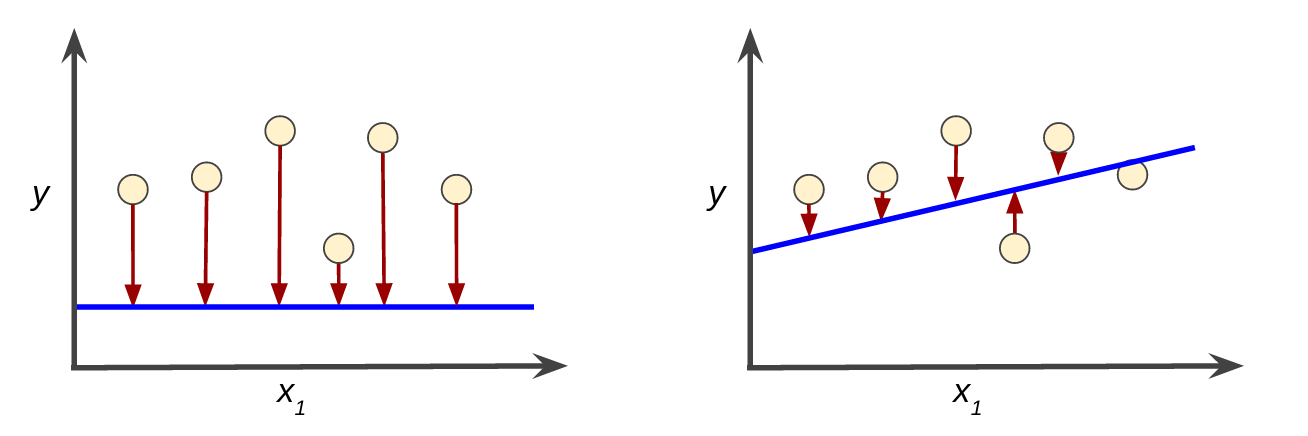
\includegraphics[width=12cm]{images/supervised/training_loss_role/LossSideBySide.png}
			%\caption{Stripe Radar for Fraud Detection}
		\end{figure}
	%\end{block}

\end{frame}


\subsubsection[$L_2$ Loss]{$L_2$ Loss}
\begin{frame}

	\frametitle{$L_2$ Loss}

	\begin{block}{}
		I modelli di regressione lineare che esamineremo utilizzano una funzione di perdita chiamata errore quadratico (nota anche come $L_2$ o Squared Loss).
		\newlinedouble
		La $L_2$ Loss per un singolo esempio è calcolato come segue:

		\begin{empheq}[box=\fcolorbox{blue!40!black!60}{yellow!10}]{align*}
		L_2 & = \text{the square of the difference between the label and the prediction}\\ & = (observation - prediction(x))^2 \\ & = (y - y')^2
		\end{empheq}

		\vspace{1mm}
	\end{block}

\end{frame}


\subsubsection[$MSE$ Loss]{$MSE$ Loss}
\begin{frame}

	\frametitle{$MSE$ Loss (Mean Squared Error)}

	%\begin{block}{}
		L'\textbf{errore quadratico medio} (MSE) è la perdita quadratica media per esempio sull'intero set di dati. Per calcolare MSE, si sommano tutti gli errori quadratici per i singoli esempi e poi si divide per il numero di esempi:

		\begin{scriptsize}
		\begin{empheq}[box=\fcolorbox{blue!40!black!60}{yellow!10}]{align*}
			MSE = \frac{1}{N} \sum_{(x,y)\in\mathcal{D}}(y-prediction(x))^2
		\end{empheq}
		\end{scriptsize}

		Dove:
		\begin{itemize}
			\item $(x, y)$ è un esempio in cui:
				\begin{itemize}
					\item[--] $x$ è l'insieme di features (ad esempio, frinii al minuto, età, sesso) che il modello utilizza per fare previsioni
					\item[--] $y$ è la label dell'esempio (in questo caso la temperatura)
				\end{itemize}
			\item $prediction(x)$ è una funzione dei pesi e del bias in combinazione con l'insieme delle features $x$
			\item $\mathcal{D}$ è un set di dati contenente molti esempi etichettati, ovvero sono coppie (x, y)
			\item $N$ è il numero di esempi in $\mathcal{D}$

			% \item Sebbene $MSE$ sia comunemente usato nell'apprendimento automatico, non è né l'unica funzione di perdita pratica né la migliore funzione di perdita per tutte le circostanze.
		\end{itemize}

	%\end{block}

\end{frame}


\begin{frame}

	\frametitle{$MSE$ Loss: un esempio grafico}

	%\begin{block}{}
		\centering
		\animategraphics[controls={play, step, stop}, height=7cm]{8.0}{images/supervised/training_loss_role/mse_linear_regression/mse_linear_regression-}{0}{45}
	%\end{block}

\end{frame}
